\documentclass{my_eth_beamer}

\usepackage{my_math_eth}

\numberwithin{equation}{section}

% -----------------------------------------------------------------------------
% this document
\title{Introduction to Survey Sampling}
\newcommand{\TITLE}{Cluster Sampling and Multistage Designs}
\newcommand{\NR}{6}
\subtitle{Part \NR: \TITLE}
\author[Tobias Schoch]{Tobias Schoch}
\date{2024}

% -----------------------------------------------------------------------------
\begin{document}

\setstretch{1.1}

\section{\TITLE}\label{sec:clus}
\setcounter{section}{\NR}
\setcounter{Bsp}{19}
\setcounter{Def}{13}
\setcounter{EinSatz}{1}

% -----------------------------------------------------------------------------
\begin{frame}
    \frametitle{Overview}
    \noindent \hspace{0.2em}\textcolor{fhnwblue}{\bfseries \NR~\TITLE~
        \textcolor{magenta}{(brief overview only)}}
    \begin{enumerate}[\NR.1]
        \item One-Stage Cluster Sampling
        \item Two-Stage and Multistage Designs
    \end{enumerate}
\end{frame}

% -----------------------------------------------------------------------------
\begin{frame}
    \begin{figure}[htb]
        \centering
        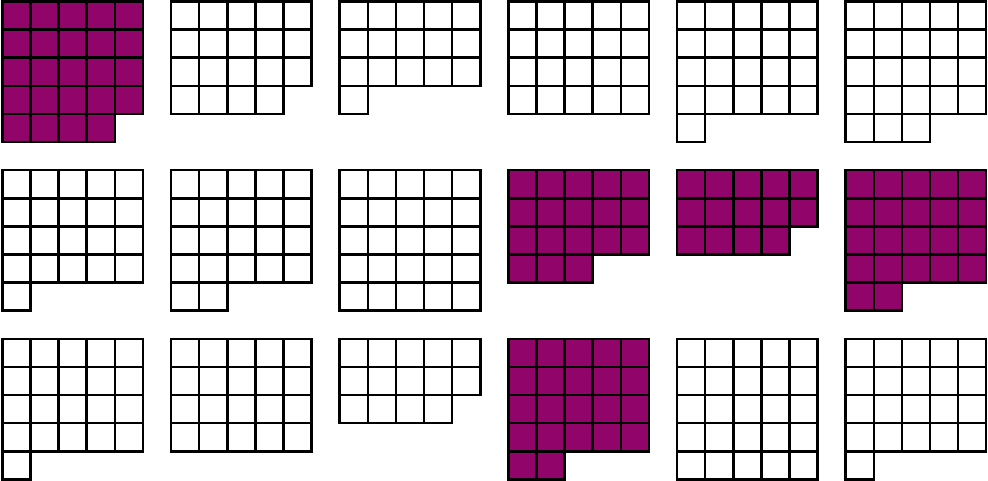
\includegraphics[width=0.9\textwidth]{figures/cluster}
        \vspace{0.5em}
        \caption{Cluster sampling: \SRS of $n=5$ from $N=18$ school classes}
        \label{fig:basics_samplingdistr}
    \end{figure}
\end{frame}

% -----------------------------------------------------------------------------
\begin{frame}
    \begin{figure}[htb]
        \centering
        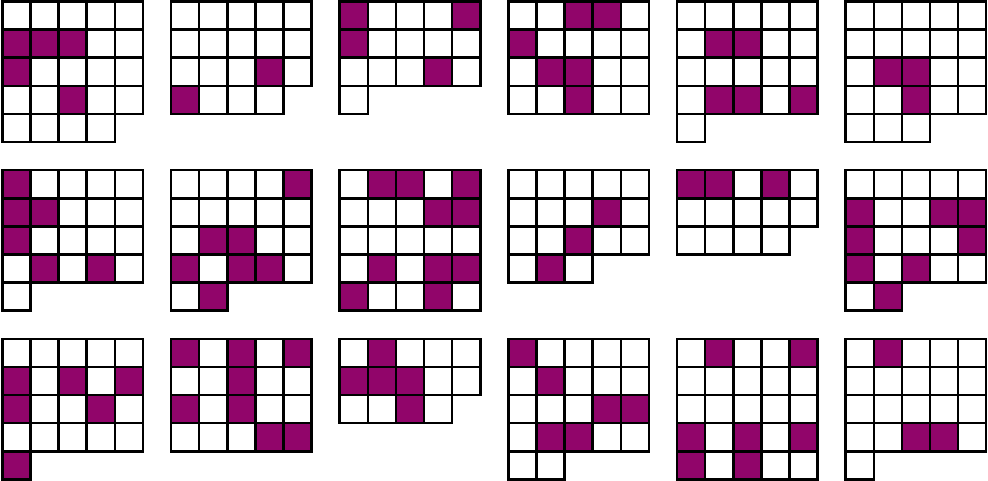
\includegraphics[width=0.9\textwidth]{figures/cluster_srs}
        \vspace{0.5em}
        \caption{Simple random sample of $n=100$ students}
        \label{fig:basics_samplingdistr}
    \end{figure}
\end{frame}

% -----------------------------------------------------------------------------
\begin{frame}
    \frametitle{\insertsectionnumber~\insertsection}
    \begin{itemize}
    \setlength{\itemsep}{6pt}
        \item \alert{Population} of school classes: $U=\{1,\ldots,18\}$
            (see example)
        \item \alert{Goal}: estimate the population total $\ty$ of
            \alert{project hours} ($y_i$) per week (focus: population;
            analyses at other levels are also possible)
        \item \alert{Procedure}:
            \vspace{0.25em}
            \begin{itemize}
            \setlength{\itemsep}{4pt}
                \item Select an \SRS of $n=5$ \alert{clusters} (school classes)
                    from $U$.
                \item Observe \alert{all elements} (students) in the selected
                    clusters (school classes).
            \end{itemize}
        \item \alert{Reasons} for using this approach:
            \vspace{0.25em}
            \begin{itemize}
            \setlength{\itemsep}{4pt}
                \item cost savings and economies of scale
                \item the cluster total may itself be of interest, e.g.,
                    total income of all persons in a household
            \end{itemize}
    \end{itemize}
\end{frame}

% -----------------------------------------------------------------------------
\begin{frame}
    \begin{itemize}
    \setlength{\itemsep}{10pt}
    \item[]
        \begin{itemize}
        \setlength{\itemsep}{2pt}
            \item constructing a sampling frame of elements may be impossible
                or too expensive (e.g., all customers in a store on a Friday
                afternoon or the number of wild boars in a region)
        \end{itemize}
        \item \alert{Clustering} and \alert{stratification} are similar in that
            both involve \alert{grouping} population elements. The sampling
            procedure, however, is different.
        \item Whereas stratification can \alert{increase precision} relative
            to \SRS, clustering generally \alert{reduces precision}.
    \end{itemize}
\end{frame}


% -----------------------------------------------------------------------------
\begin{frame}
    \noindent The notation is somewhat \alert{cumbersome}.
    \begin{align*}
        N &= \text{number of clusters in $U$}, &&
            \text{\textcolor{magenta}{number of school classes}}\\[0.75em]
        M_i &= \text{number of elements in cluster $i$} \; (i=1,\ldots,N), &&
            \text{\textcolor{magenta}{number of students in class
            $i$}}\\[0.75em]
        M_0 &= \sum_{i=1}^N M_i \; = \; \text{total number of elements},
            && \text{\textcolor{magenta}{total number of students}}\\[0.75em]
        \tyi &= \sum_{j=1}^{M_i} y_{ij} \; = \; \text{total in cluster
            $i$},&& \text{\textcolor{magenta}{total project hours in class
            $i$}}\\[0.75em]
        \ty &= \sum_{i=1}^N \tyi = \sum_{i=1}^{N}\sum_{j=1}^{M_i} y_{ij}
            \; = \; \text{population total}, &&
            \text{\textcolor{magenta}{total project hours}}\\
    \end{align*}
\end{frame}

% -----------------------------------------------------------------------------
\begin{frame}
    \begin{align*}
        \sigma_T^2 & = \frac{1}{N - 1} \sum_{i = 1}^N \left(\tyi -
            \frac{t}{N}\right)^2 = \text{var. of the cluster tot.},\\[1.55em]
        % \mt &= \frac{1}{N}\sum_{i=1}^N \tyi \; = \; \text{mean of the
        %     totals $\tyi$},\\[1em]
        \myu &= \sum_{i = 1}^N \sum_{j = 1}^{M_i} \frac{y_{ij}}{M_0} \; = \;
            \text{population mean}, &&
            \text{\textcolor{magenta}{mean number of project hours}}\\[-1em]
            & && \text{\textcolor{magenta}{per student}}\\[1em]
        \myi &= \sum_{j = 1}^{M_i} \frac{y_{ij}}{M_i} = \frac{\tyi}{M_i}
            \; = \; \text{mean in cluster $i$}, &&
            \text{\textcolor{magenta}{mean number of project hours}}\\[-1em]
            & && \text{\textcolor{magenta}{per student in class $i$}}
    \end{align*}
\end{frame}

\subsection{One-Stage Cluster Sampling}

% -----------------------------------------------------------------------------
\begin{frame}
    \frametitle{\insertsectionnumber.\insertsubsectionnumber~\insertsubsection}
    \begin{enumerate}[1)]
    \setlength{\itemsep}{6pt}
        \item Select an \SRS $s$ of $n<N$ \alert{clusters} (school classes)
            from $U$.
        \item \alert{Observe all} $M_i$ elements (students) in each cluster
            selected in Step 1, $i\in s$.
    \end{enumerate}

    \vspace{1.5em}

    \textbf{\textcolor{fhnwblue}{Estimating the population total}}

    \vspace{0.5em}

    An unbiased \alert{estimator} of $\ty$ is

    \vspace{-0.25em}

    \begin{equation*}
        \tys = N \, \mts_y, \qquad \text{with} \qquad
            \mts_y = \frac{1}{n}\sum_{i \in s} \tyi,
    \end{equation*}
    \noindent with theoretical \alert{variance}
    \begin{equation*}
        \var\big(\,\tys\big) = N^2 \left(1 - \frac{n}{N}\right)
            \frac{{\color{magenta}\bm{\sigma}_{\bm{T}}^{\bm{2}}}}{n}.
    \end{equation*}
\end{frame}

% -----------------------------------------------------------------------------
\begin{frame}
    \noindent An unbiased \alert{variance estimator} is
    \begin{equation*}
        \widehat{\var}\big(\,\tys \;\big) = N^2 \left(1 - \frac{n}{N}\right)
            \frac{\widehat{\sigma}_{\,T}^{\,2}}{n}
            \qquad \text{with} \qquad
        \widehat{\sigma}_{\,T}^{\,2} = \frac{1}{n - 1} \sum_{i \in s}
            \left(\tyi - \mts_y \, \right)^2.
    \end{equation*}

    \vspace{1.5em}

    \textbf{\textcolor{fhnwblue}{Estimating the population mean.}} We
    distinguish \alert{two cases}:

    \vspace{0.25em}

    \begin{enumerate}[1)]
    \setlength{\itemsep}{8pt}
        \item The total number of elements $M_0$ is \alert{known}. The
            population mean $\myu$ can be estimated unbiasedly by
            \begin{equation*}
                \mys_{\mathrm{\,unv}} = \frac{\tys}{M_0}, \qquad
                \text{with} \quad M_0 = \sum_{i = 1}^N M_i,
            \end{equation*}
            with \alert{variance estimator} \;
            $\widehat{\var}(\mys_{\,\mathrm{unv}}) =
                \displaystyle{\frac{\widehat{\var}(\,\tys)}{M_0^2}}$.
    \end{enumerate}
\end{frame}

% -----------------------------------------------------------------------------
\begin{frame}
    \begin{enumerate}[1)]
    \setcounter{enumi}{1}
    \setlength{\itemsep}{8pt}
        \item The total number of elements $M_0$ is \alert{unknown}. The
            population mean can be estimated by
            \begin{equation*}
                \mys_{\,\mathrm{rat}} = \frac{\sum_{i \in s} \tyi}
                    {\sum_{i \in s} M_i} = \frac{\mts_y}{\mms},
            \end{equation*}
            where $\mms$ is the sample mean of the cluster sizes $M_i$,
            $i\in s$,
            \begin{equation*}
                \mms = \frac{1}{n}\sum_{i \in s} M_i.
            \end{equation*}
            The estimator $\mys_{\,\mathrm{rat}}$ is a \alert{ratio estimator}
            and is \alert{not unbiased} for $\myu$. An approximate
            \alert{variance estimator} is
            \begin{equation*}
                \widehat{\var}(\mys_{\,\mathrm{rat}}) \approx \big(1-f\big) \,
                \frac{1}{n \, \mms^{\,2}} \, \sum_{i \in s}
                \frac{\big(t_{yi} - M_i \; \mys_{\,\mathrm{rat}}\big)^2}
                    {n - 1}.
            \end{equation*}
    \end{enumerate}
\end{frame}

% -----------------------------------------------------------------------------
\begin{frame}
    \frametitle{\normalsize{Efficiency Considerations: Design Effect}}
    \begin{itemize}
    \setlength{\itemsep}{12pt}
        \item Recall the \alert{design effect} ($\deff$) from Chapter 2.
        \item Let $U$ consist of $N$ clusters of \alert{equal size} $M$. For
            one-stage cluster sampling,
            \begin{equation*}
                \deff \approx 1+(M-1)\rho,
            \end{equation*}
            where $\rho$ is the \alert{intracluster correlation} (ICC).
        \item Typically, $\rho>0$, so that clustering results in
            \alert{deff > 1} and therefore a loss in precision relative to
            \SRS.
        \item If $\rho=0$, then $\deff\approx1$: clustering produces
            approximately the same precision as \SRS.
    \end{itemize}
\end{frame}

\subsection{Two-Stage and Multistage Designs}

% -----------------------------------------------------------------------------
\begin{frame}
    \frametitle{\insertsectionnumber.\insertsubsectionnumber~\insertsubsection}
    \begin{itemize}
    \setlength{\itemsep}{4pt}
        \item Two-stage or multistage designs select \alert{subsamples} within
            clusters. A distinction is made between \emph{multistage}
            \alert{element} and \emph{multistage} \alert{cluster}
            \emph{designs}. For a \alert{two-stage element design}, the
            procedure is as follows:
            \vspace{0.25em}
            \begin{enumerate}[1)]
            \setlength{\itemsep}{8pt}
                \item Select an \SRS $s$ of $n$ \alert{PSUs} (primary sampling
                    units; here, school classes) from $U$.
                \item Select an \SRS of \alert{SSUs} (secondary sampling units;
                    here, students) within each of the $n$ PSUs $i\in s$.
                    Denote the \SRS of $m_i$ SSUs from the $M_i$ elements by
                    $s_i$ ($i\in s$).
            \end{enumerate}
        \item The \alert{estimators} of population totals and means are
            \alert{not much more complicated} than under one-stage cluster
            sampling; see, e.g., \citet[][Chapter 3.4]{wu_thompson_2020} or
            \citet[][Chapter 5.3]{lohr_2019}.
    \end{itemize}
\end{frame}

% -----------------------------------------------------------------------------
\begin{frame}
    \begin{itemize}
    \setlength{\itemsep}{8pt}
        \item The theoretical \alert{variances}, however, are more
            \alert{complicated} because sampling occurs in two stages.
        \item \alert{Example:} Within PSU $i$, an unbiased estimator of the PSU
            total $\tyi$ is
            \begin{equation*}
                \tyis = \frac{M_i}{m_i}\sum_{j\in s_i}y_{ij}.
            \end{equation*}
        \item An unbiased estimator of the population total $\ty$ is therefore
            \begin{equation*}
                \tys = \frac{N}{n}\sum_{i\in s}\tyis.
            \end{equation*}
        \item Equivalently,
            \begin{equation*}
                \tys = \sum_{i\in s}\sum_{j\in s_i}w_{ij}y_{ij},
                \qquad w_{ij}=\frac{N M_i}{n m_i} = \frac{1}{(n/N)(m_i/M_i)}.
            \end{equation*}
    \end{itemize}
\end{frame}

% -----------------------------------------------------------------------------
\begin{frame}
    \begin{itemize}
    \setlength{\itemsep}{6pt}
        \item The \alert{theoretical} variance is
            \begin{equation*}
                \var\big(\,\tys\big) =
                    \underbrace{N^2 \left(1 - \frac{n}{N}\right)
                        \frac{\sigma_{T}^{2}}{n}}_{\text{Stage 1}} +
                    \color{magenta}\underbrace{\color{black}\frac{N}{n}
                        \sum_{i = 1}^{N}
                        \left(1 - \frac{m_i}{M_i}\right) M_i^2
                        \frac{\sigma_{yi}^2}{m_i}}_
                        {\text{\color{magenta} Stage 2}}\color{black},
            \end{equation*}
            where $\sigma_{yi}^2$ is the population variance of $y$ within
            PSU $i$.
        \item \alert{Stage 1:} uncertainty from selecting the PSUs and
            equals the variance under one-stage cluster
                    sampling.
        \item \alert{Stage 2:} additional uncertainty from subsampling
            elements within the selected PSUs.
            \vspace{0.25em}
            \begin{itemize}
            \setlength{\itemsep}{8pt}
                \item[\goto] It is small when the
                    within-PSU sampling fractions $m_i/M_i$ are large and/or
                    the within-PSU variances $\sigma_{yi}^2$ are small.
                    If all elements in each selected PSU are sampled
                    ($m_i=M_i$), the Stage 2 component is zero.
            \end{itemize}
    \end{itemize}
\end{frame}

% -----------------------------------------------------------------------------
\begin{frame}
    \begin{itemize}
    \setlength{\itemsep}{12pt}
        \item The variance estimator follows the same \alert{two-component
            structure} as the theoretical variance:
            \begin{equation*}
                \widehat{\var}(\tys)
                =
                \widehat V_{\text{Stage 1}}
                +
                \widehat V_{\text{Stage 2}}.
            \end{equation*}
            \item The \alert{Stage 1} component is estimated from the
                variability of the estimated PSU totals $\tyis$ across the
                sampled PSUs
                \vspace{0.25em}
                \begin{itemize}
                \setlength{\itemsep}{8pt}
                    \item[\goto] It uses the estimated PSU totals $\tyis$, not
                        the unknown true totals $\tyi$.
                \end{itemize}
            \item The \alert{Stage 2} component is estimated from the
                within-PSU sample variances $\widehat{\sigma}_{yi}^2$ in the
                sampled PSUs.
    \end{itemize}
\end{frame}

% -----------------------------------------------------------------------------
\begin{frame}
    \frametitle{\normalsize{Multistage and Multiphase Designs}}
    \begin{itemize}
    \setlength{\itemsep}{12pt}
        \item \alert{Multistage sampling:} sampling proceeds through a
            \alert{hierarchy} of sampling units. For example, first sample
            schools (PSUs), then students (SSUs) within the sampled schools.
            \vspace{0.25em}
            \begin{itemize}
            \setlength{\itemsep}{8pt}
                \item[\goto] Second-stage samples are typically selected
                    independently across PSUs, which simplifies variance
                    calculations.
            \end{itemize}
    \item \alert{Multiphase sampling:} essentially the same type of units
        is sampled in successive phases, typically because different
        information is collected at different phases. For example, draw a
        large first-phase sample and collect inexpensive auxiliary
        variables, then select a subsample for more costly measurements.
    \end{itemize}
\end{frame}

% -----------------------------------------------------------------------------
\setcounter{section}{\the\numexpr\value{section}-1\relax}
\begin{frame}
    \frametitle{References}
    {\footnotesize
        \setstretch{1.1}
        \bibliographystyle{fhnw_en}
        \bibliography{master}
    }
\end{frame}

% -----------------------------------------------------------------------------
\lastpage

\end{document}
